\section{Protocol and implementation details}
\label{app:protocol}
\subsection{Models and extraction}
The standalone references are DINOv2-L \citep{oquab2024dinov2} and
SigLIP2-so400m-patch14-384 \citep{tschannen2025siglip2}. The extracted pipelines come
from Kimi K2.6, Kimi K3, Muse Glimmer 30B, and Qwen3.8-27B
\citep{moonshot2026kimik26,moonshot2026kimik3,meta2026museglimmer,qwen2026qwen38}.
The repository adapters record their standalone checkpoint identifiers. The Qwen
result filenames retain the internal slug \texttt{qwen3\_5}; their recorded model ID
identifies the Qwen3.8 checkpoint evaluated here. Likewise, \texttt{moonvit\_v2}
identifies the Kimi K3 tower. Display names in this paper follow the recorded models.

At $448\times448$, patch-14 towers produce 1,024 tokens and Qwen3.8 produces 784.
Merging concatenates each $2\times2$ block, reducing these counts to 256 and 196 while
quadrupling feature width. The merged widths are 4,608 for Kimi K2.6 and Qwen3.8,
4,096 for Kimi K3, and 6,144 for Muse Glimmer. Native normalization and packing are
preserved; SigLIP2's position grid is interpolated from its configured resolution.
Qwen tower tokens are restored from merge-block order to raster order, and intermediate
Muse Glimmer tokens from attention-window order to raster order, before spatial scoring.

Extraction tests check exact parent weight equality for 335 packaged Kimi K2.6 tensors,
809 Muse Glimmer tensors, and 333 Qwen3.8 tensors, with parent stage-output comparisons.
Kimi K3 has equality checks for its 165 tower tensors. Its three exported projector
tensors are checked for compatible shapes, not equality to a separately loaded parent
projector; there is no parent forward-output comparison. These different validation
levels apply to every result that uses the respective adapter. Cache-level lossless-merge
checks cover Kimi K2.6 and Kimi K3; losslessness for the other two is inferred from the
implemented architecture.

\subsection{Datasets and spatial alignment}
ImageNet-100 uses the 13,000-image \texttt{validation} split of
\texttt{ilee0022/ImageNet100} \citep{ilee0022imagenet100}, exported by
\texttt{scripts/export\_imagenet100.py} and split with a fixed seed into
9,100/1,950/1,950 training/validation/test images. We identify the exact export because
ImageNet-100 does not designate a unique class list or split. The four label budgets subsample only
the training split and retain every class. Pooling to 16 tokens reduces recognition
cache storage; the full-token validation is described in Appendix~\ref{app:corrections}.

DIODE uses 771 validation-release images with normals, comprising 325 indoor and
446 outdoor images. The 541/115/115 split is fixed. Native $768\times1024$ images are
center-cropped consistently with the tower input; depth and normal targets retain their
native resolution within that crop. The observed depth range sets the head's bin ceiling
to 299.83\,m. A Probe3D-style multiscale decoder \citep{elbanani2024probe3d,ranftl2021dpt}
reads one layer, rather than combining four encoder layers. We train for 10 epochs with
AdamW \citep{loshchilov2019adamw}, batch size eight. The records also contain
$\delta_2$, $\delta_3$, RMSE, and scene-specific metrics. This single-layer, DIODE-based
protocol differs from the original Probe3D evaluation.

KITTI uses the selected-validation archive of the depth-completion dataset, partitioned
700/150/150. Readouts receive RGB features only; sparse depth provides targets.
Unsigned 16-bit depth is decoded in units of $1/256$\,m, zeros remain invalid, and
invalid pixels are masked in loss and evaluation. Mean valid coverage is 17.08\%, and
the recorded maximum depth is 85.766\,m. All towers use final tower features, with
projected features additionally evaluated for the four connectors, in the matched arm.

NAVI uses 555 wild-set pairs with relative rotations in $(0,120]$ degrees. ScanNet uses
1,500 pairs from the SuperGlue test split \citep{sarlin2020superglue}. SPair-71k samples
up to 200 pairs in each of 18 classes, for 3,600 pairs; the projected-versus-tower
intervals use 3,408 pairs with finite scores at both stages. NAVI and ScanNet features
are bicubically resized to $64\times64$ before cosine nearest-neighbor matching;
Lowe's ratio \citep{lowe2004distinctive} ranks up to 1,000 retained matches. ScanNet RGB
is aligned to the depth/intrinsics frame before cropping. SPair bilinearly samples
source features at annotated keypoints, then selects target grid centers by cosine argmax.
It uses each stage's own grid: $32\times32$ or $28\times28$ at the tower, and
$16\times16$ or $14\times14$ after merging/projection. It uses neither Lowe ranking nor
a top-1,000 cutoff. The SPair records' \texttt{evaluation\_side: 64} field is unused by
that scoring path. These protocols are adaptations of Probe3D. SPair aggregate levels are class-macro averages where labeled; bootstrap
contrasts average paired image-pair differences and use a different weighting.

Occlusion uses a fixed 2,000-image ImageNet-100 subset, with 300 held-out test images.
The reducer and attention readout are fitted on clean training features and frozen for
all masking conditions. Records include requested and actual occluded area, rectangle
coordinates, and fill value. Object scale and blur were planned but not measured.

\subsection{Readout capacity and learning rates}
Mean recognition averages tokens before a linear classifier. Attention recognition uses
a learned query, a 512-wide multihead projection, layer normalization, and a classifier.
The matched PCA arm fits the reduction on each cell's training features only, then
freezes it. Parameter counts after reduction are 51,300 for mean recognition,
1,627,748 for attention recognition, 1,444,608 for depth, and 1,314,819 for normals.
Raw heads grow with feature width. Matching parameter count does not ensure equal
optimization difficulty or equal representation distortion.

Recognition searches
$\{10^{-5},3\cdot10^{-5},10^{-4},3\cdot10^{-4},10^{-3},3\cdot10^{-3},
10^{-2},3\cdot10^{-2},10^{-1},3\cdot10^{-1},1\}$;
geometry searches
$\{10^{-4},3\cdot10^{-4},10^{-3},3\cdot10^{-3},10^{-2},3\cdot10^{-2}\}$.
The selected rate maximizes validation accuracy or depth $\delta_1$, or minimizes
validation normal error, as appropriate. Three retraining seeds provide the reported
mean and population standard deviation. Paired image bootstrap intervals
\citep{efron1993bootstrap} average over those seeds before resampling, preserving the
pairing between the two extraction points on each image.

\section{Protocol corrections and pooling control}
\label{app:corrections}
The initial recognition grid began at $3\cdot10^{-4}$. Of 224 cells, 107 chose that
floor: 53 of 56 matched-attention cells and 54 of 56 raw-attention cells, with no mean
cells choosing it. The original run also had three upper-limit selections, for 110
boundary selections overall. After grid expansion and deterministic PCA correction,
three selections remain at a boundary, all DINOv2 raw-mean cells at the upper limit. The experiment now records the
complete validation search rather than only the selected rate.

Separately, randomized PCA originally depended on process RNG history. The reducer now
seeds its randomized SVD inside a forked random-number context, leaving readout RNG
state unchanged. All 112 matched recognition cells were rerun. Compared with the
previous randomized matched run, 18 selected another learning rate; mean absolute top-1
changes were 0.00270 for attention and 0.00310 for mean pooling. The largest changes
were $-0.0110$ for DINOv2 attention and $+0.0156$ for SigLIP2 mean pooling.

The original Muse Glimmer matched-attention merge-to-projector difference was
$-0.0075$ top-1; the corrected result is $+0.0042$. Both learning-rate selection and
PCA changed, so this contrast cannot isolate either correction's contribution.
It also should not be described as a reversed paired significance test: the original
claim used seed spread. The corrected attention stage changes are small and do not
establish a general recognition gain or loss from projection.

The original matched geometry matrix cannot be reconstructed exactly because the PCA
draws were not saved. Headline geometry comparisons were therefore retrained under the
deterministic reducer; their point estimates can differ from the descriptive matrix.
Recognition bootstrap comparisons also use separately retrained runs and can differ
slightly from matrix or label-budget means. A bootstrap difference must be read from
its own result record, not reconstructed by subtracting rounded entries in Table~\ref{tab:capability}.

Pooling validation compares SigLIP2 and Muse Glimmer on a 1,500-image subset cached
with both full tokens and $4\times4$ pooling. It covers both readouts and capacity
arms. Mean readout rankings and curves agree, with raw means matching to four decimals.
Six of sixteen full-token attention cells collapse at intermediate layers, preventing
validation of the pooled attention curves. Diagnostics vary dataset size and training
length on three unstable cells. With 5,000 images and 20 epochs, SigLIP2 matched at
relative depth 0.630 scores $0.6796\pm0.1551$; extending training to 100 epochs stabilizes
the two matched cells but leaves SigLIP2 raw at $0.7227\pm0.0275$. No tested configuration
meets the stability target across all three cells. The records support an inconclusive
attention-pooling control, not proof that pooling is harmless or that it causes the gap.

\section{Geometry layer peaks}
\label{app:peaks}
Table~\ref{tab:peaks} reports every geometry curve's best observed test score and its
cost at the final layer. For depth the cost is peak minus final $\delta_1$; for normals
it is final minus minimum angular error. These maxima and minima are selected from the
test sweep, not a separate validation selection. The matched arm uses the original
randomized-PCA matrix. The single final-layer geometry peak is DINOv2 raw depth.

\begin{table}[H]
\centering\small
\caption{Descriptive geometry peaks across both capacity arms. Depth scores and costs
are $\delta_1$; normal scores and costs are degrees.}
\label{tab:peaks}
\begin{tabular}{lllrrr}
\toprule
Tower & Task & Arm & Peak depth & Peak score & Final-layer cost\\
\midrule
DINOv2 & Depth & matched & 0.875 & 0.7015 & 0.0256\\
SigLIP2 & Depth & matched & 0.630 & 0.6702 & 0.0764\\
Muse Glimmer & Depth & matched & 0.760 & 0.6588 & 0.1227\\
Kimi K2.6 & Depth & matched & 0.519 & 0.6595 & 0.0593\\
Qwen3.8 & Depth & matched & 0.630 & 0.6736 & 0.1422\\
Kimi K3 & Depth & matched & 0.630 & 0.6546 & 0.1167\\
DINOv2 & Normals & matched & 0.750 & 18.8508 & 4.3426\\
SigLIP2 & Normals & matched & 0.370 & 23.9039 & 7.1108\\
Muse Glimmer & Normals & matched & 0.620 & 24.3014 & 7.2328\\
Kimi K2.6 & Normals & matched & 0.370 & 25.5109 & 5.1786\\
Qwen3.8 & Normals & matched & 0.370 & 24.2386 & 10.2153\\
Kimi K3 & Normals & matched & 0.370 & 27.0277 & 4.7317\\
DINOv2 & Depth & raw & 1.000 & 0.6746 & 0.0000\\
SigLIP2 & Depth & raw & 0.519 & 0.6366 & 0.0546\\
Muse Glimmer & Depth & raw & 0.620 & 0.6035 & 0.1946\\
Kimi K2.6 & Depth & raw & 0.741 & 0.5089 & 0.0446\\
Qwen3.8 & Depth & raw & 0.630 & 0.6439 & 0.3001\\
Kimi K3 & Depth & raw & 0.630 & 0.5440 & 0.0878\\
DINOv2 & Normals & raw & 0.750 & 19.4649 & 2.7510\\
SigLIP2 & Normals & raw & 0.370 & 25.1602 & 5.4407\\
Muse Glimmer & Normals & raw & 0.620 & 22.7825 & 11.0423\\
Kimi K2.6 & Normals & raw & 0.889 & 30.3440 & 1.7705\\
Qwen3.8 & Normals & raw & 0.519 & 24.6806 & 9.0479\\
Kimi K3 & Normals & raw & 0.630 & 27.9684 & 5.3326\\
\bottomrule
\end{tabular}

\end{table}

\section{Paired comparisons}
\label{app:intervals}
All tables in this section are generated from the paired result JSONs. Intervals are
pointwise 95\% bootstrap intervals with 10,000 resamples. Positive advantages favor the
first representation. For normal error, the sign is reversed so positive means lower
error. Each table uses its stated evaluation unit and capacity setting.

\subsection{DIODE}
The following two tables cover all 16 projected-versus-final-tower comparisons on
115 images. Depth uses $\delta_1$ and normals use degrees of error reduction.
DINOv2 and SigLIP2 have no native projected stage and are not included.

\begin{table}[H]
\centering\small
\caption{DIODE projected-versus-tower differences, matched arm.}
\label{tab:projector}
\begin{tabular}{llrr}
\toprule
Connector & Task & Difference & 95\% interval\\
\midrule
Kimi K2.6 & Depth & $+0.0174$ & $[+0.0060, +0.0289]$\\
Kimi K3 & Depth & $+0.0784$ & $[+0.0596, +0.0984]$\\
Muse Glimmer & Depth & $+0.0261$ & $[+0.0129, +0.0395]$\\
Qwen3.8 & Depth & $+0.0584$ & $[+0.0374, +0.0809]$\\
Kimi K2.6 & Normals & $+2.1980$ & $[+1.6538, +2.7685]$\\
Kimi K3 & Normals & $+2.4968$ & $[+1.9616, +3.0492]$\\
Muse Glimmer & Normals & $+0.7924$ & $[+0.3770, +1.2065]$\\
Qwen3.8 & Normals & $+4.3130$ & $[+3.3956, +5.3018]$\\
\bottomrule
\end{tabular}

\end{table}
\begin{table}[H]
\centering\small
\caption{DIODE projected-versus-tower differences, raw arm.}
\begin{tabular}{llrr}
\toprule
Connector & Task & Difference & 95\% interval\\
\midrule
Kimi K2.6 & Depth & $+0.0196$ & $[-0.0003, +0.0402]$\\
Kimi K3 & Depth & $+0.0270$ & $[+0.0113, +0.0427]$\\
Muse Glimmer & Depth & $+0.0927$ & $[+0.0624, +0.1237]$\\
Qwen3.8 & Depth & $+0.1601$ & $[+0.1211, +0.1977]$\\
Kimi K2.6 & Normals & $+3.1126$ & $[+2.4215, +3.8228]$\\
Kimi K3 & Normals & $+2.8269$ & $[+2.1506, +3.5442]$\\
Muse Glimmer & Normals & $+2.8932$ & $[+2.3767, +3.4432]$\\
Qwen3.8 & Normals & $+4.4432$ & $[+3.5076, +5.4427]$\\
\bottomrule
\end{tabular}

\end{table}

Scene-specific intervals for the matched arm use 51 indoor and 64 outdoor images.
Fifteen of these sixteen intervals exclude zero; Kimi K2.6 outdoor depth is unresolved.

\begin{table}[H]
\centering\small
\caption{DIODE projected-versus-tower differences by scene, matched arm.}
\begin{tabular}{lllrr}
\toprule
Connector & Task & Scene & Difference & 95\% interval\\
\midrule
Kimi K2.6 & Depth & Indoor & $+0.0325$ & $[+0.0145, +0.0506]$\\
Kimi K2.6 & Depth & Outdoor & $+0.0053$ & $[-0.0085, +0.0198]$\\
Kimi K3 & Depth & Indoor & $+0.1170$ & $[+0.0813, +0.1541]$\\
Kimi K3 & Depth & Outdoor & $+0.0476$ & $[+0.0333, +0.0643]$\\
Muse Glimmer & Depth & Indoor & $+0.0336$ & $[+0.0099, +0.0584]$\\
Muse Glimmer & Depth & Outdoor & $+0.0201$ & $[+0.0064, +0.0347]$\\
Qwen3.8 & Depth & Indoor & $+0.0499$ & $[+0.0153, +0.0858]$\\
Qwen3.8 & Depth & Outdoor & $+0.0651$ & $[+0.0393, +0.0930]$\\
Kimi K2.6 & Normals & Indoor & $+3.2144$ & $[+2.2093, +4.2502]$\\
Kimi K2.6 & Normals & Outdoor & $+1.3880$ & $[+0.8998, +1.9298]$\\
Kimi K3 & Normals & Indoor & $+3.5815$ & $[+2.6695, +4.5369]$\\
Kimi K3 & Normals & Outdoor & $+1.6324$ & $[+1.1034, +2.2109]$\\
Muse Glimmer & Normals & Indoor & $+1.1128$ & $[+0.3023, +1.9190]$\\
Muse Glimmer & Normals & Outdoor & $+0.5372$ & $[+0.1624, +0.9161]$\\
Qwen3.8 & Normals & Indoor & $+6.8576$ & $[+5.2091, +8.6752]$\\
Qwen3.8 & Normals & Outdoor & $+2.2853$ & $[+1.7216, +2.8849]$\\
\bottomrule
\end{tabular}

\end{table}

\subsection{KITTI and correspondence}
KITTI differences use $\delta_1$, matched readouts, and 150 test images. Correspondence
has no trained head or capacity arm: NAVI uses recall at 2\,cm over 555 pairs, ScanNet
recall at 10 pixels over 1,500 pairs, and SPair PCK at 0.1 over 3,408 finite pairs.
SPair differences weight pairs equally, rather than weighting classes equally.

\begin{table}[H]
\centering\small
\caption{KITTI projected-versus-tower differences.}
\label{tab:kitti}
\begin{tabular}{lrr}
\toprule
Connector & Difference & 95\% interval\\
\midrule
Kimi K2.6 & $-0.0048$ & $[-0.0077, -0.0016]$\\
Kimi K3 & $+0.0014$ & $[-0.0011, +0.0038]$\\
Muse Glimmer & $-0.0039$ & $[-0.0074, -0.0007]$\\
Qwen3.8 & $-0.0021$ & $[-0.0053, +0.0012]$\\
\bottomrule
\end{tabular}

\end{table}
\begin{table}[H]
\centering\small
\caption{NAVI projected-versus-tower differences.}
\begin{tabular}{lrr}
\toprule
Connector & Difference & 95\% interval\\
\midrule
Kimi K2.6 & $+0.0565$ & $[+0.0521, +0.0609]$\\
Kimi K3 & $+0.0590$ & $[+0.0542, +0.0637]$\\
Muse Glimmer & $+0.1058$ & $[+0.0995, +0.1121]$\\
Qwen3.8 & $+0.0188$ & $[+0.0146, +0.0230]$\\
\bottomrule
\end{tabular}

\end{table}
\begin{table}[H]
\centering\small
\caption{ScanNet projected-versus-tower differences.}
\begin{tabular}{lrr}
\toprule
Connector & Difference & 95\% interval\\
\midrule
Kimi K2.6 & $+0.0075$ & $[+0.0061, +0.0090]$\\
Kimi K3 & $+0.0213$ & $[+0.0202, +0.0225]$\\
Muse Glimmer & $+0.0318$ & $[+0.0299, +0.0336]$\\
Qwen3.8 & $-0.0194$ & $[-0.0208, -0.0180]$\\
\bottomrule
\end{tabular}

\end{table}
\begin{table}[H]
\centering\small
\caption{SPair-71k projected-versus-tower differences.}
\begin{tabular}{lrr}
\toprule
Connector & Difference & 95\% interval\\
\midrule
Kimi K2.6 & $+0.1150$ & $[+0.1063, +0.1235]$\\
Kimi K3 & $-0.0144$ & $[-0.0216, -0.0070]$\\
Muse Glimmer & $+0.1325$ & $[+0.1239, +0.1411]$\\
Qwen3.8 & $+0.0216$ & $[+0.0118, +0.0316]$\\
\bottomrule
\end{tabular}

\end{table}

\subsection{Recognition and cross-tower geometry}
Recognition comparisons include both between-tower and within-Qwen layer contrasts,
all paired over 1,950 test images. Each representation is labeled by its relative depth.
The matched attention Muse Glimmer--DINOv2 contrast and both raw Qwen earlier-layer
contrasts exclude zero. The remaining recognition intervals cross zero.

\begin{table}[H]
\centering\scriptsize
\caption{Recognition differences, first minus second top-1 accuracy.}
\begin{tabular}{lllrr}
\toprule
First / second & Readout & Arm & Difference & 95\% interval\\
\midrule
Muse Glimmer 1.000 / DINOv2 1.000 & attention & matched & $+0.0125$ & $[+0.0034, +0.0215]$\\
Muse Glimmer 1.000 / SigLIP2 1.000 & attention & matched & $+0.0041$ & $[-0.0036, +0.0121]$\\
Qwen3.8 0.741 / Qwen3.8 1.000 & attention & matched & $+0.0017$ & $[-0.0063, +0.0096]$\\
SigLIP2 1.000 / DINOv2 1.000 & attention & matched & $+0.0084$ & $[-0.0009, +0.0178]$\\
Muse Glimmer 1.000 / SigLIP2 1.000 & attention & raw & $-0.0017$ & $[-0.0097, +0.0063]$\\
Qwen3.8 0.889 / Qwen3.8 1.000 & attention & raw & $+0.0128$ & $[+0.0053, +0.0203]$\\
Muse Glimmer 1.000 / SigLIP2 1.000 & mean & matched & $-0.0039$ & $[-0.0130, +0.0053]$\\
Qwen3.8 0.889 / Qwen3.8 1.000 & mean & matched & $+0.0015$ & $[-0.0056, +0.0085]$\\
Muse Glimmer 1.000 / SigLIP2 1.000 & mean & raw & $-0.0010$ & $[-0.0104, +0.0085]$\\
Qwen3.8 0.889 / Qwen3.8 1.000 & mean & raw & $+0.0156$ & $[+0.0053, +0.0263]$\\
\bottomrule
\end{tabular}

\end{table}

The two cross-tower geometry comparisons rerun test-sweep-selected layers with
deterministic PCA: depth at relative depths 0.875 for DINOv2 and 0.630 for Qwen3.8,
and normals at 0.750 for DINOv2 and 0.370 for SigLIP2. Layer selection has no independent
validation. DINOv2--Qwen3.8 depth compares different native grids; DINOv2--SigLIP2 normals
uses the same token count. The rerun depth levels are 0.6988 and 0.6697; normal errors
are 18.8204 and 23.8575 degrees. They need not equal the original sweep's values.

\begin{table}[H]
\centering\small
\caption{Cross-tower geometry advantages under deterministic matched reruns.}
\begin{tabular}{llrr}
\toprule
First / second & Task & Advantage & 95\% interval\\
\midrule
DINOv2 / Qwen3.8 & Depth & $+0.0292$ & $[+0.0099, +0.0484]$\\
DINOv2 / SigLIP2 & Normals & $+5.0370$ & $[+4.3038, +5.8164]$\\
\bottomrule
\end{tabular}

\end{table}

\section{Occlusion and correspondence levels}
\label{app:secondary}
Figure~\ref{fig:secondary} shows absolute occluded-image accuracy and NAVI scores through
the connector. Its occlusion panel is not a clean-minus-perturbed difference.
Within-stage clean-versus-occluded intervals resolve a loss at 10\% masking for all
multimodal stages. DINOv2's tower is unresolved at that level and first resolves at
20\%. The apparent cross-tower retention groups have not been tested with paired
retention intervals. No connector stage is uniformly more resistant to occlusion.

The NAVI panel illustrates the scoring effect of merging. Qwen3.8, Kimi K2.6, and
Muse Glimmer fall after concatenation and recover after projection. This demonstrates
format sensitivity of direct cosine matching; the numerical size of that fall is not
a bound on information loss or recovery in the adjacent stage.

\begin{figure}[H]
\centering
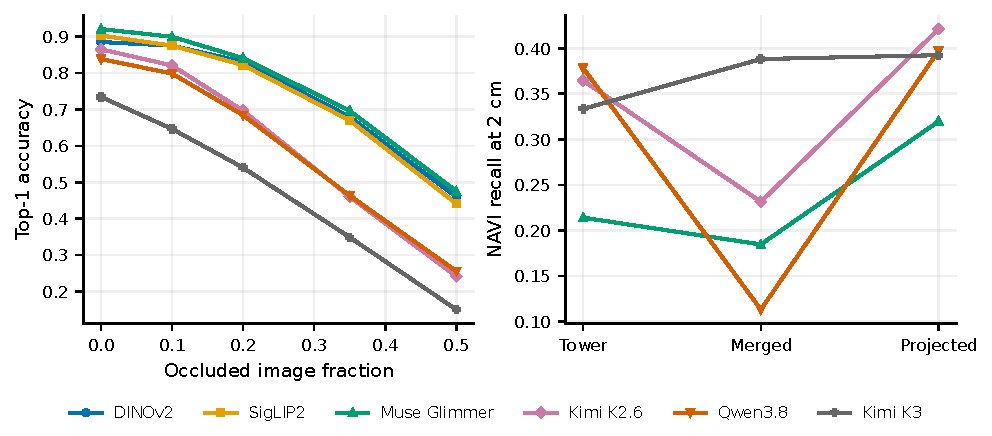
\includegraphics[width=0.9\textwidth]{figures/paper-secondary.pdf}
\caption{Left: absolute top-1 accuracy under occlusion at the tower stage, matched
attention readout. Right: training-free NAVI recall at the three native stages for
multimodal towers. Curves are descriptive; uncertainty is not plotted.}
\label{fig:secondary}
\end{figure}

\begin{table}[H]
\centering\small
\caption{Final-tower correspondence levels. SPair is a macro average over 18 classes;
its paired intervals above average over finite image pairs instead.}
\label{tab:correspondence}
\begin{tabular}{lrrr}
\toprule
Tower & NAVI & ScanNet & SPair (macro)\\
\midrule
DINOv2 & 0.5389 & 0.0896 & 0.5547\\
SigLIP2 & 0.4013 & 0.0584 & 0.3982\\
Muse Glimmer & 0.2139 & 0.0208 & 0.0909\\
Kimi K2.6 & 0.3646 & 0.0547 & 0.1782\\
Qwen3.8 & 0.3785 & 0.0834 & 0.3081\\
Kimi K3 & 0.3334 & 0.0258 & 0.2760\\
\bottomrule
\end{tabular}

\end{table}

\section{Result provenance and reproduction}
Source and results: \url{https://github.com/immanuel-peter/vision-tower-bench}.
Build instructions are in \texttt{paper/README.md}.
\texttt{paper/build\_assets.py} generates numerical assets from recorded JSONs, with input
hashes in \texttt{paper/asset-sources.json}.
\texttt{results/README.md} indexes the experiments and corrections.
